% Options for packages loaded elsewhere
\PassOptionsToPackage{unicode}{hyperref}
\PassOptionsToPackage{hyphens}{url}
\PassOptionsToPackage{dvipsnames,svgnames,x11names}{xcolor}
%
\documentclass[
  letterpaper,
  DIV=11,
  numbers=noendperiod]{scrartcl}

\usepackage{amsmath,amssymb}
\usepackage{iftex}
\ifPDFTeX
  \usepackage[T1]{fontenc}
  \usepackage[utf8]{inputenc}
  \usepackage{textcomp} % provide euro and other symbols
\else % if luatex or xetex
  \usepackage{unicode-math}
  \defaultfontfeatures{Scale=MatchLowercase}
  \defaultfontfeatures[\rmfamily]{Ligatures=TeX,Scale=1}
\fi
\usepackage{lmodern}
\ifPDFTeX\else  
    % xetex/luatex font selection
\fi
% Use upquote if available, for straight quotes in verbatim environments
\IfFileExists{upquote.sty}{\usepackage{upquote}}{}
\IfFileExists{microtype.sty}{% use microtype if available
  \usepackage[]{microtype}
  \UseMicrotypeSet[protrusion]{basicmath} % disable protrusion for tt fonts
}{}
\makeatletter
\@ifundefined{KOMAClassName}{% if non-KOMA class
  \IfFileExists{parskip.sty}{%
    \usepackage{parskip}
  }{% else
    \setlength{\parindent}{0pt}
    \setlength{\parskip}{6pt plus 2pt minus 1pt}}
}{% if KOMA class
  \KOMAoptions{parskip=half}}
\makeatother
\usepackage{xcolor}
\setlength{\emergencystretch}{3em} % prevent overfull lines
\setcounter{secnumdepth}{-\maxdimen} % remove section numbering
% Make \paragraph and \subparagraph free-standing
\makeatletter
\ifx\paragraph\undefined\else
  \let\oldparagraph\paragraph
  \renewcommand{\paragraph}{
    \@ifstar
      \xxxParagraphStar
      \xxxParagraphNoStar
  }
  \newcommand{\xxxParagraphStar}[1]{\oldparagraph*{#1}\mbox{}}
  \newcommand{\xxxParagraphNoStar}[1]{\oldparagraph{#1}\mbox{}}
\fi
\ifx\subparagraph\undefined\else
  \let\oldsubparagraph\subparagraph
  \renewcommand{\subparagraph}{
    \@ifstar
      \xxxSubParagraphStar
      \xxxSubParagraphNoStar
  }
  \newcommand{\xxxSubParagraphStar}[1]{\oldsubparagraph*{#1}\mbox{}}
  \newcommand{\xxxSubParagraphNoStar}[1]{\oldsubparagraph{#1}\mbox{}}
\fi
\makeatother


\providecommand{\tightlist}{%
  \setlength{\itemsep}{0pt}\setlength{\parskip}{0pt}}\usepackage{longtable,booktabs,array}
\usepackage{calc} % for calculating minipage widths
% Correct order of tables after \paragraph or \subparagraph
\usepackage{etoolbox}
\makeatletter
\patchcmd\longtable{\par}{\if@noskipsec\mbox{}\fi\par}{}{}
\makeatother
% Allow footnotes in longtable head/foot
\IfFileExists{footnotehyper.sty}{\usepackage{footnotehyper}}{\usepackage{footnote}}
\makesavenoteenv{longtable}
\usepackage{graphicx}
\makeatletter
\def\maxwidth{\ifdim\Gin@nat@width>\linewidth\linewidth\else\Gin@nat@width\fi}
\def\maxheight{\ifdim\Gin@nat@height>\textheight\textheight\else\Gin@nat@height\fi}
\makeatother
% Scale images if necessary, so that they will not overflow the page
% margins by default, and it is still possible to overwrite the defaults
% using explicit options in \includegraphics[width, height, ...]{}
\setkeys{Gin}{width=\maxwidth,height=\maxheight,keepaspectratio}
% Set default figure placement to htbp
\makeatletter
\def\fps@figure{htbp}
\makeatother

\KOMAoption{captions}{tableheading}
\makeatletter
\@ifpackageloaded{tcolorbox}{}{\usepackage[skins,breakable]{tcolorbox}}
\@ifpackageloaded{fontawesome5}{}{\usepackage{fontawesome5}}
\definecolor{quarto-callout-color}{HTML}{909090}
\definecolor{quarto-callout-note-color}{HTML}{0758E5}
\definecolor{quarto-callout-important-color}{HTML}{CC1914}
\definecolor{quarto-callout-warning-color}{HTML}{EB9113}
\definecolor{quarto-callout-tip-color}{HTML}{00A047}
\definecolor{quarto-callout-caution-color}{HTML}{FC5300}
\definecolor{quarto-callout-color-frame}{HTML}{acacac}
\definecolor{quarto-callout-note-color-frame}{HTML}{4582ec}
\definecolor{quarto-callout-important-color-frame}{HTML}{d9534f}
\definecolor{quarto-callout-warning-color-frame}{HTML}{f0ad4e}
\definecolor{quarto-callout-tip-color-frame}{HTML}{02b875}
\definecolor{quarto-callout-caution-color-frame}{HTML}{fd7e14}
\makeatother
\makeatletter
\@ifpackageloaded{caption}{}{\usepackage{caption}}
\AtBeginDocument{%
\ifdefined\contentsname
  \renewcommand*\contentsname{Table of contents}
\else
  \newcommand\contentsname{Table of contents}
\fi
\ifdefined\listfigurename
  \renewcommand*\listfigurename{List of Figures}
\else
  \newcommand\listfigurename{List of Figures}
\fi
\ifdefined\listtablename
  \renewcommand*\listtablename{List of Tables}
\else
  \newcommand\listtablename{List of Tables}
\fi
\ifdefined\figurename
  \renewcommand*\figurename{Figure}
\else
  \newcommand\figurename{Figure}
\fi
\ifdefined\tablename
  \renewcommand*\tablename{Table}
\else
  \newcommand\tablename{Table}
\fi
}
\@ifpackageloaded{float}{}{\usepackage{float}}
\floatstyle{ruled}
\@ifundefined{c@chapter}{\newfloat{codelisting}{h}{lop}}{\newfloat{codelisting}{h}{lop}[chapter]}
\floatname{codelisting}{Listing}
\newcommand*\listoflistings{\listof{codelisting}{List of Listings}}
\makeatother
\makeatletter
\makeatother
\makeatletter
\@ifpackageloaded{caption}{}{\usepackage{caption}}
\@ifpackageloaded{subcaption}{}{\usepackage{subcaption}}
\makeatother

\ifLuaTeX
  \usepackage{selnolig}  % disable illegal ligatures
\fi
\usepackage{bookmark}

\IfFileExists{xurl.sty}{\usepackage{xurl}}{} % add URL line breaks if available
\urlstyle{same} % disable monospaced font for URLs
\hypersetup{
  pdftitle={A Reproducible Paper},
  pdfauthor={Elijah Knaap; Another Person},
  pdfkeywords={reproducibility, open science},
  colorlinks=true,
  linkcolor={blue},
  filecolor={Maroon},
  citecolor={Blue},
  urlcolor={Blue},
  pdfcreator={LaTeX via pandoc}}


\title{A Reproducible Paper\thanks{This project is supported by the
National Science Foundation Grant \#2345820: An Open Source Ecosystem
for Spatial Data Science.}}
\usepackage{etoolbox}
\makeatletter
\providecommand{\subtitle}[1]{% add subtitle to \maketitle
  \apptocmd{\@title}{\par {\large #1 \par}}{}{}
}
\makeatother
\subtitle{Using \texttt{pixi} and \texttt{quarto} and codespaces to
handle environments and execution}
\author{Elijah Knaap \and Another Person}
\date{2024-11-21}

\begin{document}
\maketitle
\begin{abstract}
This project shows how to generate a reproducible environment and
execute an entire analysis (including building the paper) via github
codespaces.
\end{abstract}


\section{Introduction}\label{introduction}

\section{Literature Review}\label{literature-review}

\section{Methods}\label{methods}

Two classic models in spatial analysis are the \emph{Spatial Lag Model},
defined as

\[y = \rho Wy + \beta X + \epsilon\]

and the \emph{Spatial Error Model} defined as

\[
\begin{split}
y & = \beta X + u\\
u & = \lambda W u + \epsilon
\end{split}
\]

\section{Results}\label{results}

This section uses \texttt{quarto}'s conditional formatting to swap out
the correct table depending out output. The problem here is
\texttt{pandas} can write nice latex tables, but those don't convert to
html. Instead you can just write both formats out to file and select the
correct one on-demand.

\begin{longtable}{lrr}
\caption{Blockgroups in San Diego} \\
\toprule
 & n-total-pop & median-household-income \\
\midrule
\endfirsthead
\caption[]{Blockgroups in San Diego} \\
\toprule
 & n-total-pop & median-household-income \\
\midrule
\endhead
\midrule
\multicolumn{3}{r}{Continued on next page} \\
\midrule
\endfoot
\bottomrule
\endlastfoot
0 & 1577.000000 & 150688.000000 \\
1 & 1673.000000 & 127292.000000 \\
2 & 1915.000000 & 90673.000000 \\
3 & 1271.000000 & 65219.000000 \\
4 & 695.000000 & NaN \\
5 & 2617.000000 & 81250.000000 \\
6 & 500.000000 & 64631.000000 \\
7 & 808.000000 & 64787.000000 \\
8 & 1682.000000 & 59010.000000 \\
9 & 1151.000000 & 79725.000000 \\
\end{longtable}

You can also do the same thing with figures, e.g.~to swap in an
interactive map in the html output and use a static map in the pdf.

\begin{figure}

\centering{

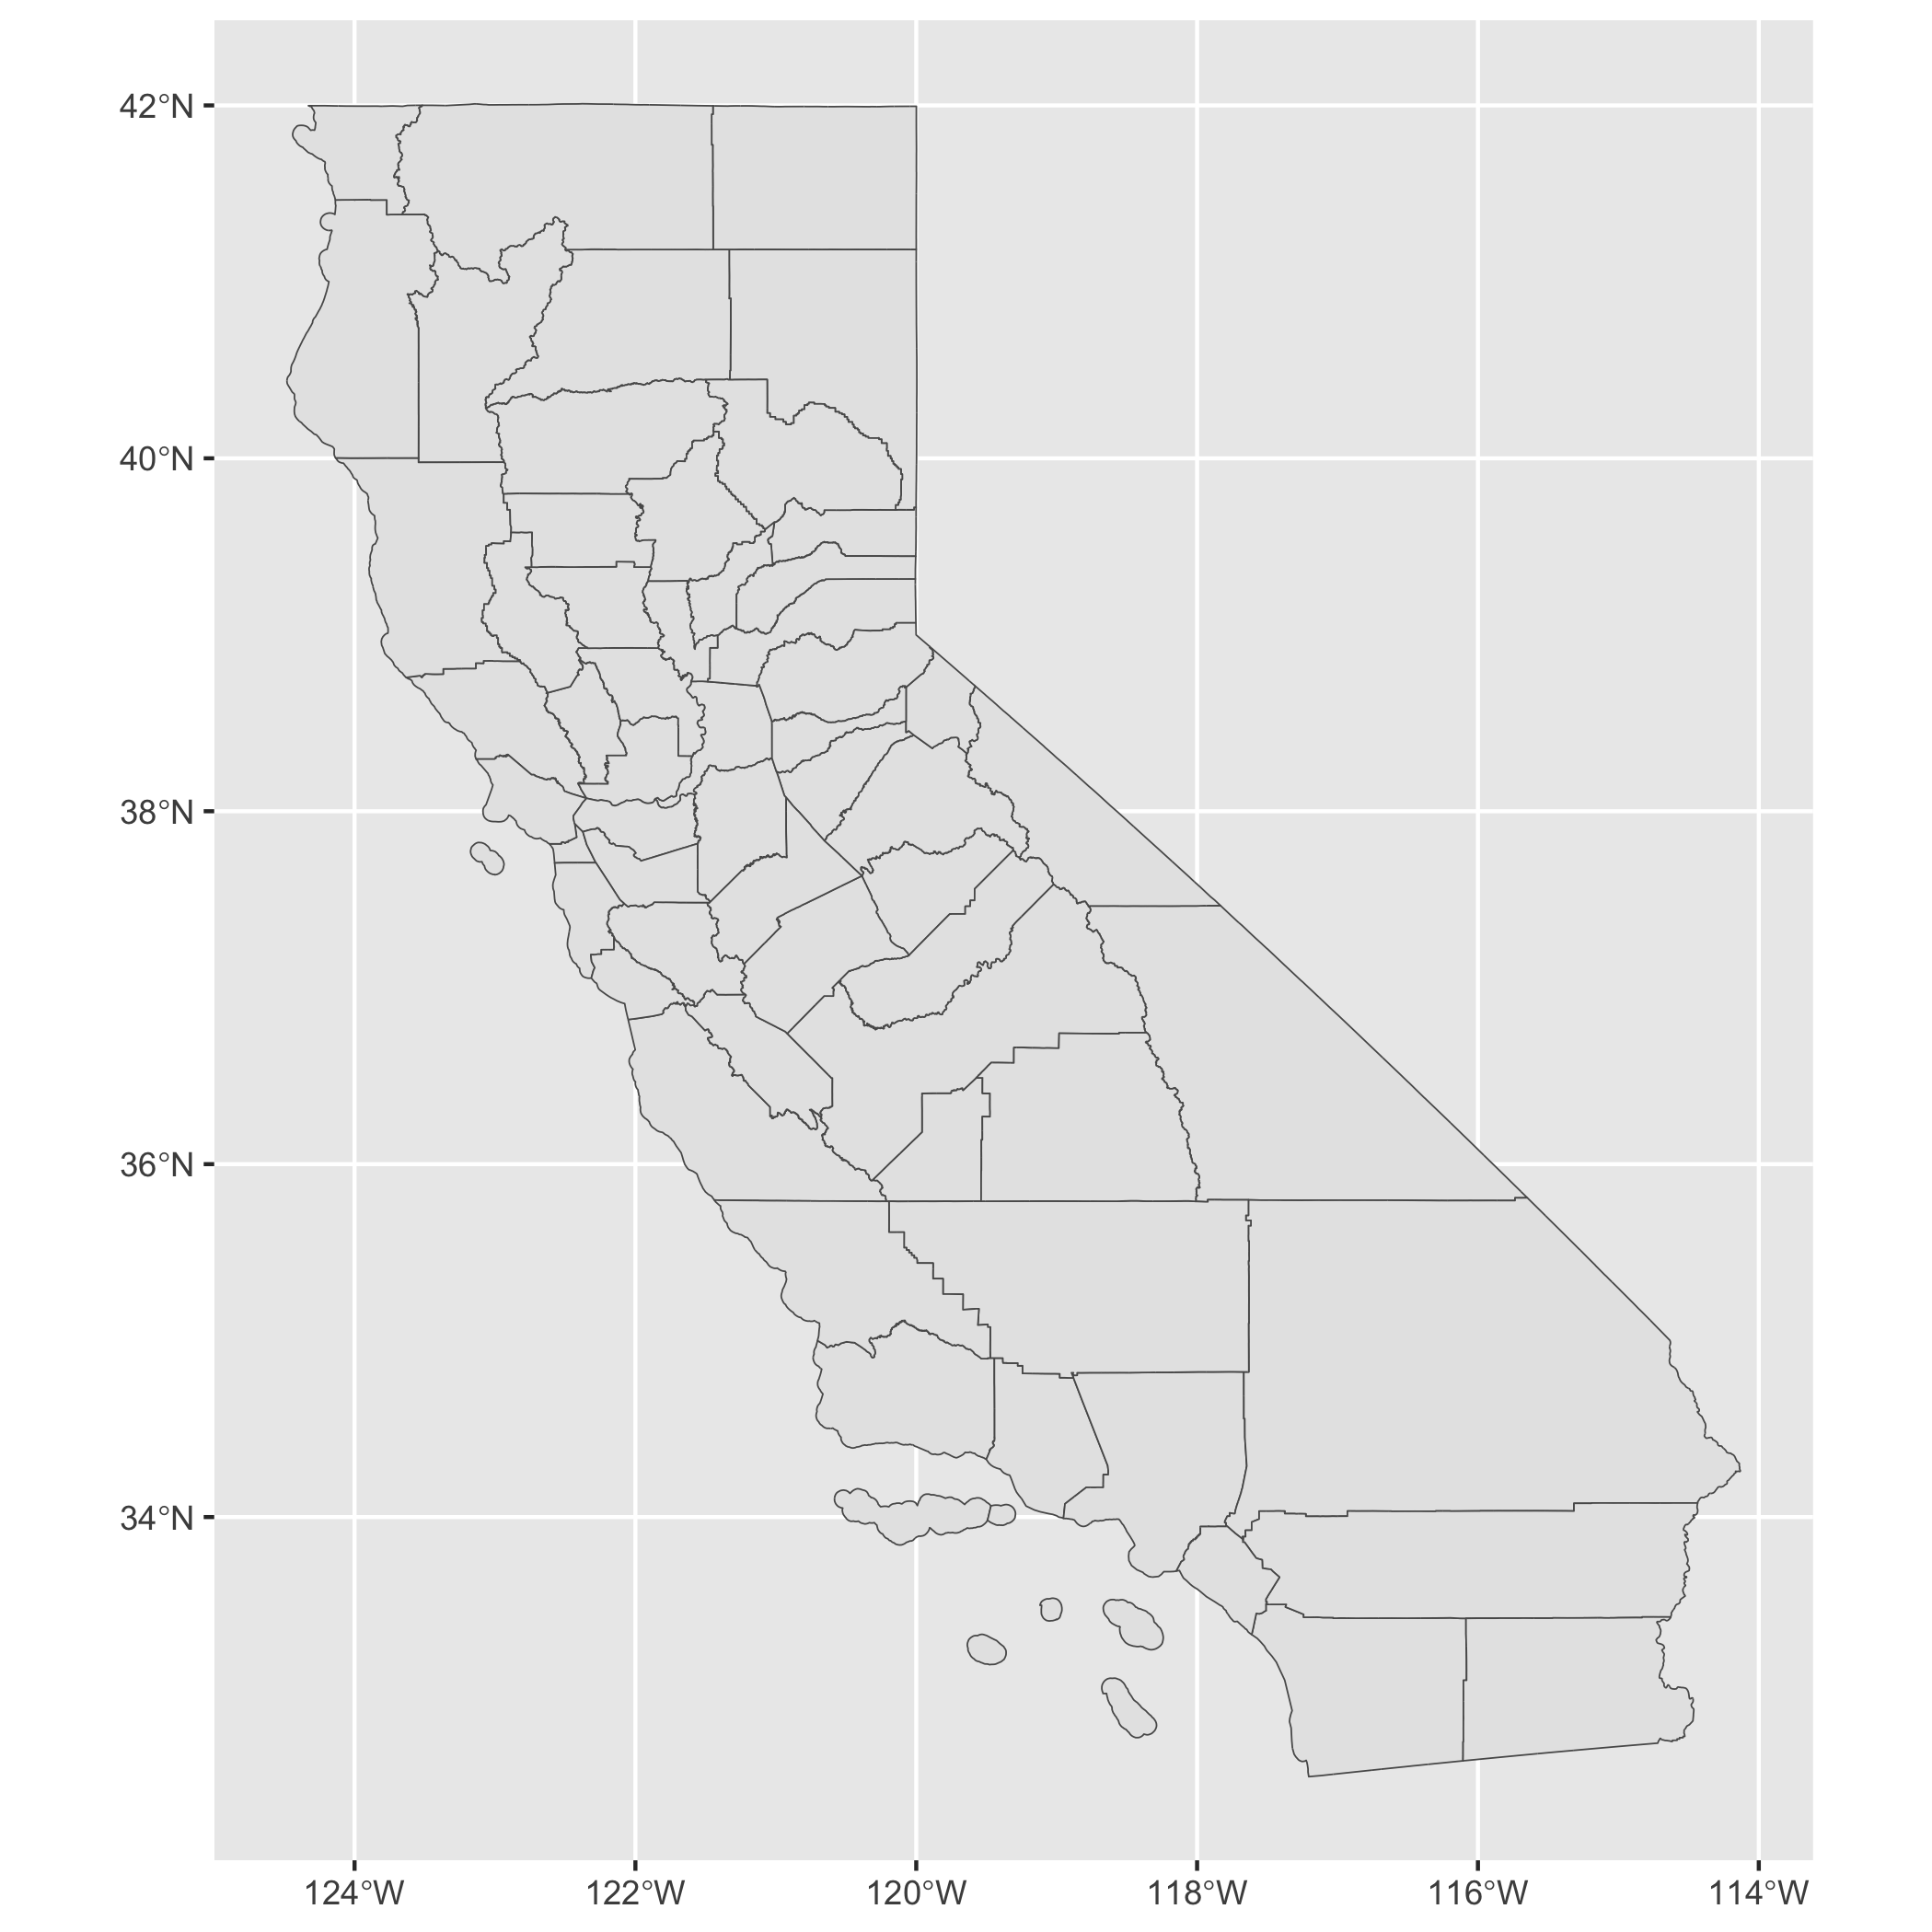
\includegraphics[width=0.6\textwidth,height=\textheight]{_fig_ggmap.png}

}

\caption{\label{fig-counties}California Counties}

\end{figure}%

Everyone from the \texttt{R} world will recognize this figure as coming
from \texttt{ggplot}. It shows up either way. But the blockgroups in San
Diego show up differently depending on the output.

\begin{figure}

\centering{

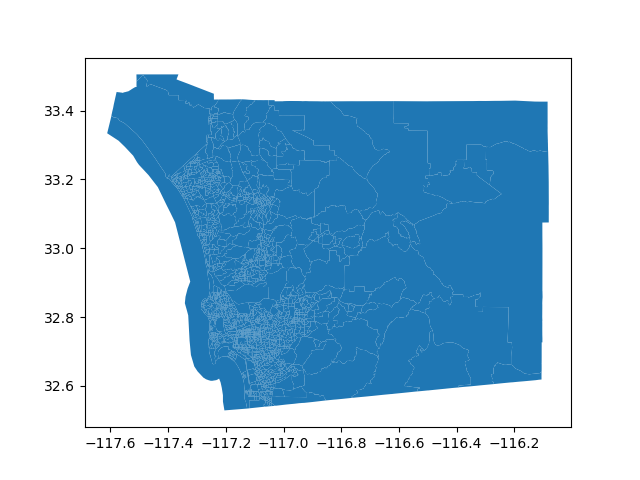
\includegraphics{_fig_sdmap.png}

}

\caption{\label{fig-sdmap}SD Map}

\end{figure}%

\begin{tcolorbox}[enhanced jigsaw, colframe=quarto-callout-note-color-frame, breakable, leftrule=.75mm, arc=.35mm, opacityback=0, titlerule=0mm, colback=white, bottomrule=.15mm, toprule=.15mm, opacitybacktitle=0.6, bottomtitle=1mm, coltitle=black, toptitle=1mm, colbacktitle=quarto-callout-note-color!10!white, title=\textcolor{quarto-callout-note-color}{\faInfo}\hspace{0.5em}{Note}, rightrule=.15mm, left=2mm]

This is kinda hacky because it relies on an iFrame that requires the
embedded map to be available the relative URL set above (you cant
download this html file and expect it to work). The
\texttt{embed-resources} option in quarto wont work for an iframe
either.

\end{tcolorbox}

\section{Discussion}\label{discussion}

\section{Conclusion}\label{conclusion}

\section{References}\label{references}




\end{document}
